\subsection{Case01 - Drop}
\label{p4_wifi_case01}

En este caso de uso se probará que es posible descartar todos los paquetes recibidos con un programa P4 en una interfaz virtual \textit{Wireless}. Como tal el programa P4 no es suficiente para probar esta funcionalidad ya que requiere de una plataforma que sea capaz de soportar el lenguaje P4. Se hará uso de software switch llamado behavioral-model, \gls{bmv2} en adelante, para testear los programas P4, y de la integración desarrollada anteriormente con Mininet-WiFi como escenario para recrear las topologías de Red.\\
\par

Como este caso de uso ya se ha explicado anteriormente en el case01 de P4 cableado (Ver subsección \ref{p4_ether_case01}), y no hay ninguna diferencia inducida en el cambio de entorno según se explico en las sección anterior,  únicamente se harán indicaciones sobre como poder compilarlo y ejecutarlo. Importante, si usted está replicando este caso de uso, sin antes haber adecuado las dependencias necesarias de Mininet-WiFi con soporte del \gls{bmv2}, vuelva a este punto \ref{mn_wifi_own_deps} y siga los pasos indicados.

% figura escenario
\begin{figure}[ht]
    \centering
    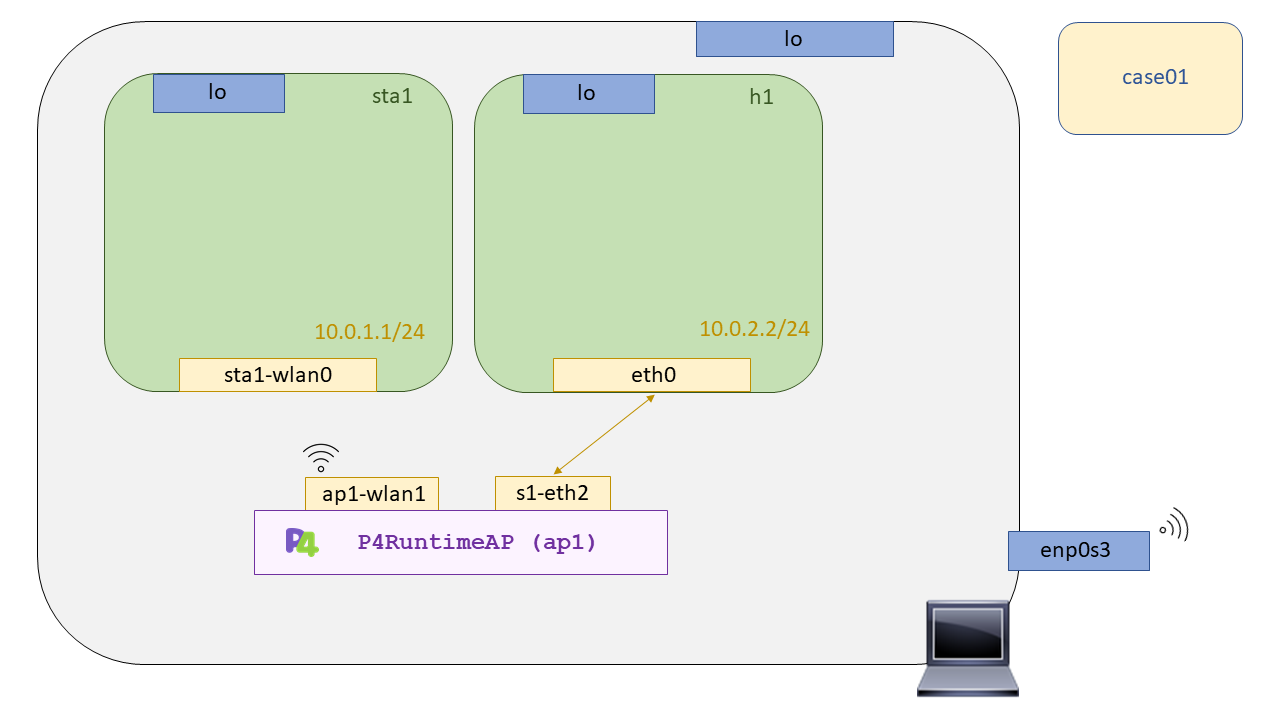
\includegraphics[width=16cm]{archivos/img/dev/p4-wifi/case01/scenario.png}
    \caption{Escenario del Case01 - P4 Wireless}
    \label{fig:case01_p4_wifi_scenario}
\end{figure}

\vspace{0.2cm}
\textbf{Compilación}\\
\par

Para la compilación de este caso de uso, se ha dejado preparado un Makefile, por tanto no es necesario que el usuario aprenda a utilizar el compilador p4c. Si se quiere saber más sobre como funciona el proceso de compilación, qué etapas hay, como se le "inyecta" el \texttt{json} generado al \gls{bmv2}, o qué distintos \textit{targets} hay en función de la arquitectura, le recomendamos que vuelva al case01 (\ref{p4_ether_case01}). Para llevar a cabo la compilación solo se tendrá que seguir los pasos indicados en el bloque \ref{code:case01_p4_wifi_load}.

\begin{lstlisting}[language= bash, style=Consola, caption={Compilación programa P4  - Case01},label=code:case01_p4_wifi_load]
    # Entramos al directorio 
    cd TFG/src/use_cases/p4-wireless/case01

    # Hacemos uso del Makefile
    sudo make
\end{lstlisting}
\vspace{0.5cm}


Una vez ejecutado el make, se habrá generado una estructura de directorios que se utilizarán en el lanzamiento del caso de uso. Bajo el directorio \texttt{build} se podrá encontrar el \texttt{json} generado por el compilador, será este \texttt{json} quien tenga toda la información requerida para conformar el \gls{bmv2}.\\
\par

\vspace{0.2cm}
\textbf{Puesta en marcha del escenario}\\
\par

Al igual que en la compilación, se ha dejado preparado un script en Python para automatizar la puesta en marcha del escenario. Este script describe la topología que se utilizará en este caso de uso. Recordemos que es necesario volver hacer un \texttt{make install} para instalar los módulos adicionales generados para la integración del \gls{bmv2} y Mininet-WiFi, además de tener instaladas las versiones indicadas en el análisis de la integración. Estas dependencias se pueden encontrar en el apartado \ref{mn_wifi_own_deps} \\
\par

Una vez comprobado que posee todas la dependencias, simplemente se tendrá que ejecutar el script con el interprete de Python. Este script levantará la topología descrita en la figura \ref{fig:case01_p4_wifi_scenario}, compuesto por dos hosts y por una instancia del nodo \texttt{P4RuntimeAP}. El nodo \texttt{ap1}, del tipo \texttt{P4RuntimeAP}, tendrá dos interfaces, una wireless y un par de \gls{veth}.



\begin{lstlisting}[language= bash, style=Consola, caption={Puesta en marcha del escenario  - Case01},label=code:case01_p4_wifi_run]
    sudo python scenario.py
\end{lstlisting}
\vspace{0.2cm}


\vspace{0.5cm}
\textbf{Comprobación del funcionamiento}\\
\par

Tras las ejecución del script \texttt{scenario.py}, se tendría el escenario \ref{fig:case01_p4_wifi_scenario} levantado, y la CLI de Mininet-WiFi abierta. Para la comprobación de funcionamiento de este caso de uso, se van a seguir los mismos pasos que en el case01 (\ref{p4_ether_case01}) - P4 en un entorno alámbrico. Por tanto no se entrará en hacer explicaciones que se creen redundantes, se indicarán los pasos seguidos para llevar a cabo la comprobación de funcionamiento y los resultados de dichas pruebas. 

\begin{lstlisting}[language= bash, style=Consola, caption={Pasos a seguir para comprobar el funcionamiento - Case01},label=code:case01_p4_wifi_func1]
    mininet-wifi>  xterm sta1 h1
    
    # Se hará ping desde la estación Wifi al Host
    [sta1] ping 10.0.2.2
    
    
    # Se pondrá a escuchar en el Host
    [h1] tcpdump -l

\end{lstlisting}
\vspace{0.5cm}


% Figura
% figura escenario
\begin{figure}[ht]
    \centering
    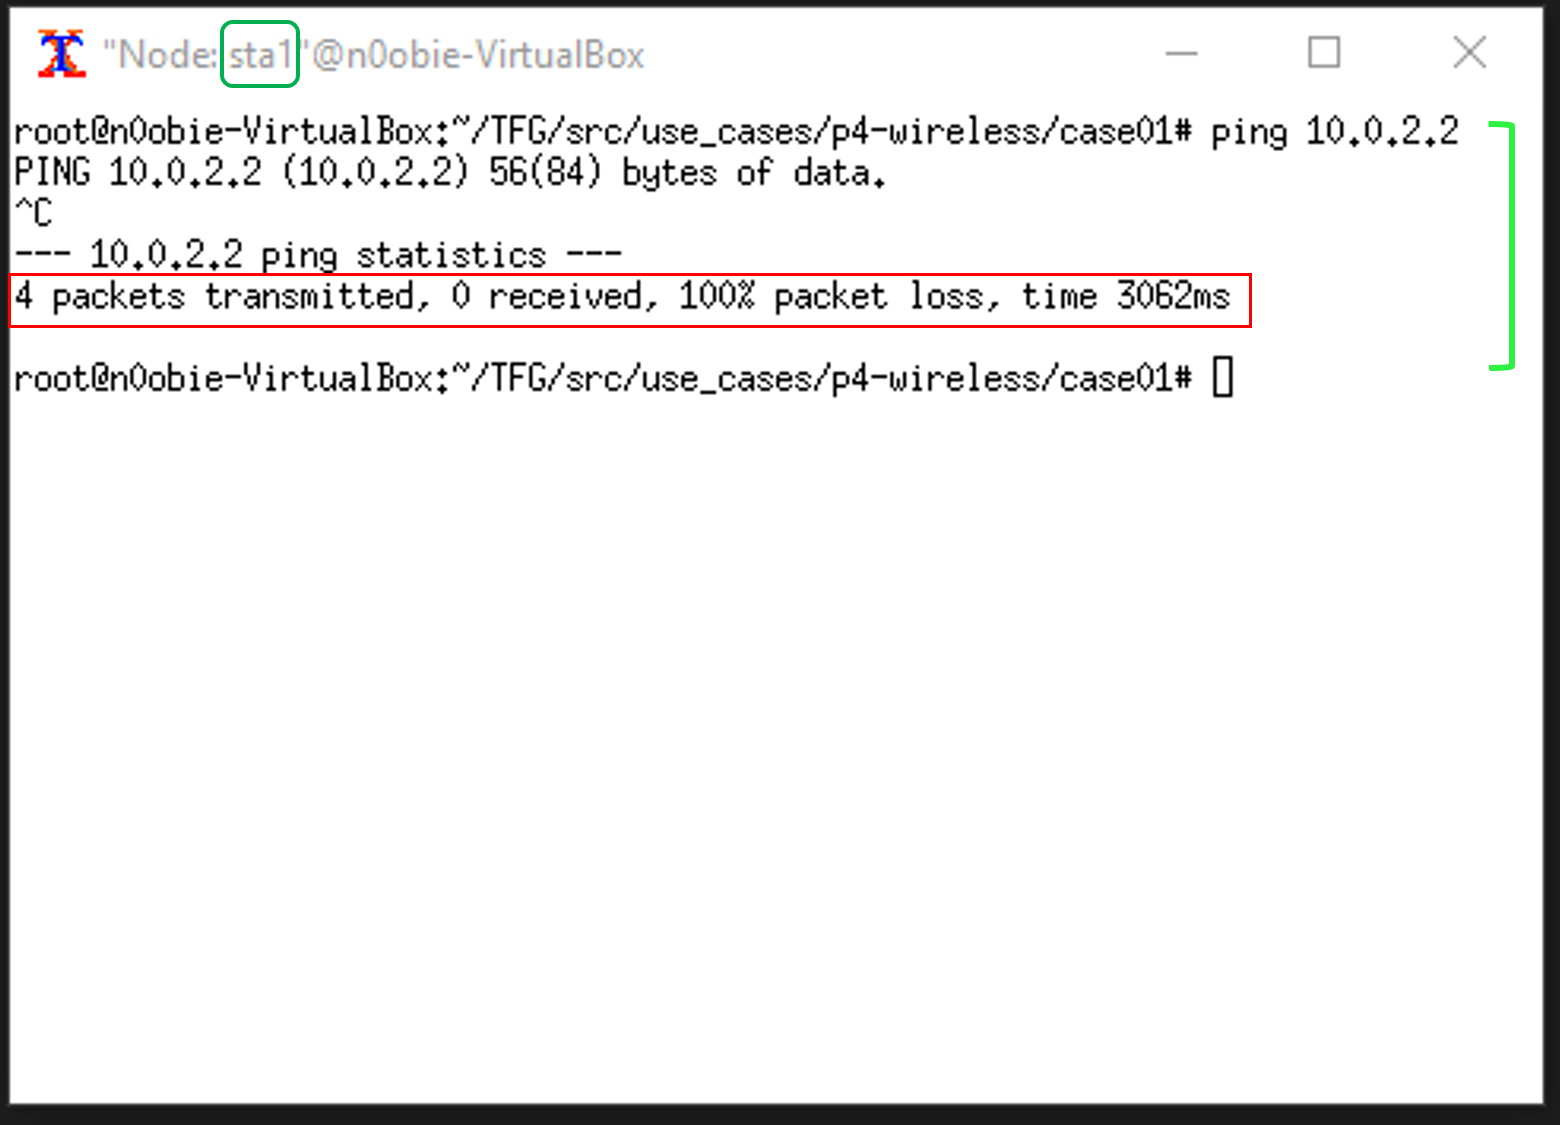
\includegraphics[width=14cm]{archivos/img/dev/p4-wifi/case01/demo_case01_1_edited.png}
    \caption{Comprobación de funcionamiento (Ping) del Case01 - P4 Wireless}
    \label{fig:case01_p4_wifi_func1}
\end{figure}
\vspace{0.5cm}

Como se puede ver en la figura \ref{fig:case01_p4_wifi_func1}, no hay conectividad entre ambos nodos dado que el ping \fcolorbox{black}{green}{\rule{0pt}{2.5pt}\rule{2.5pt}{0pt}}\hspace{1mm} no está llegando. Por lo que, el programa P4 está funcionando según lo esperado, tirando los paquetes que llegan a su \textit{pipeline} de procesamiento. Para asegurarse de que realmente se está ejecutando el \textit{action} para tirar paquetes podemos consultar los logs del \gls{bmv2}, los cuales generan un fichero de log por cada instancia \textit{target} del \texttt{P4RuntimeAP} que se haya levantado.\\
\par

\newpage

\begin{figure}[ht]
    \centering
    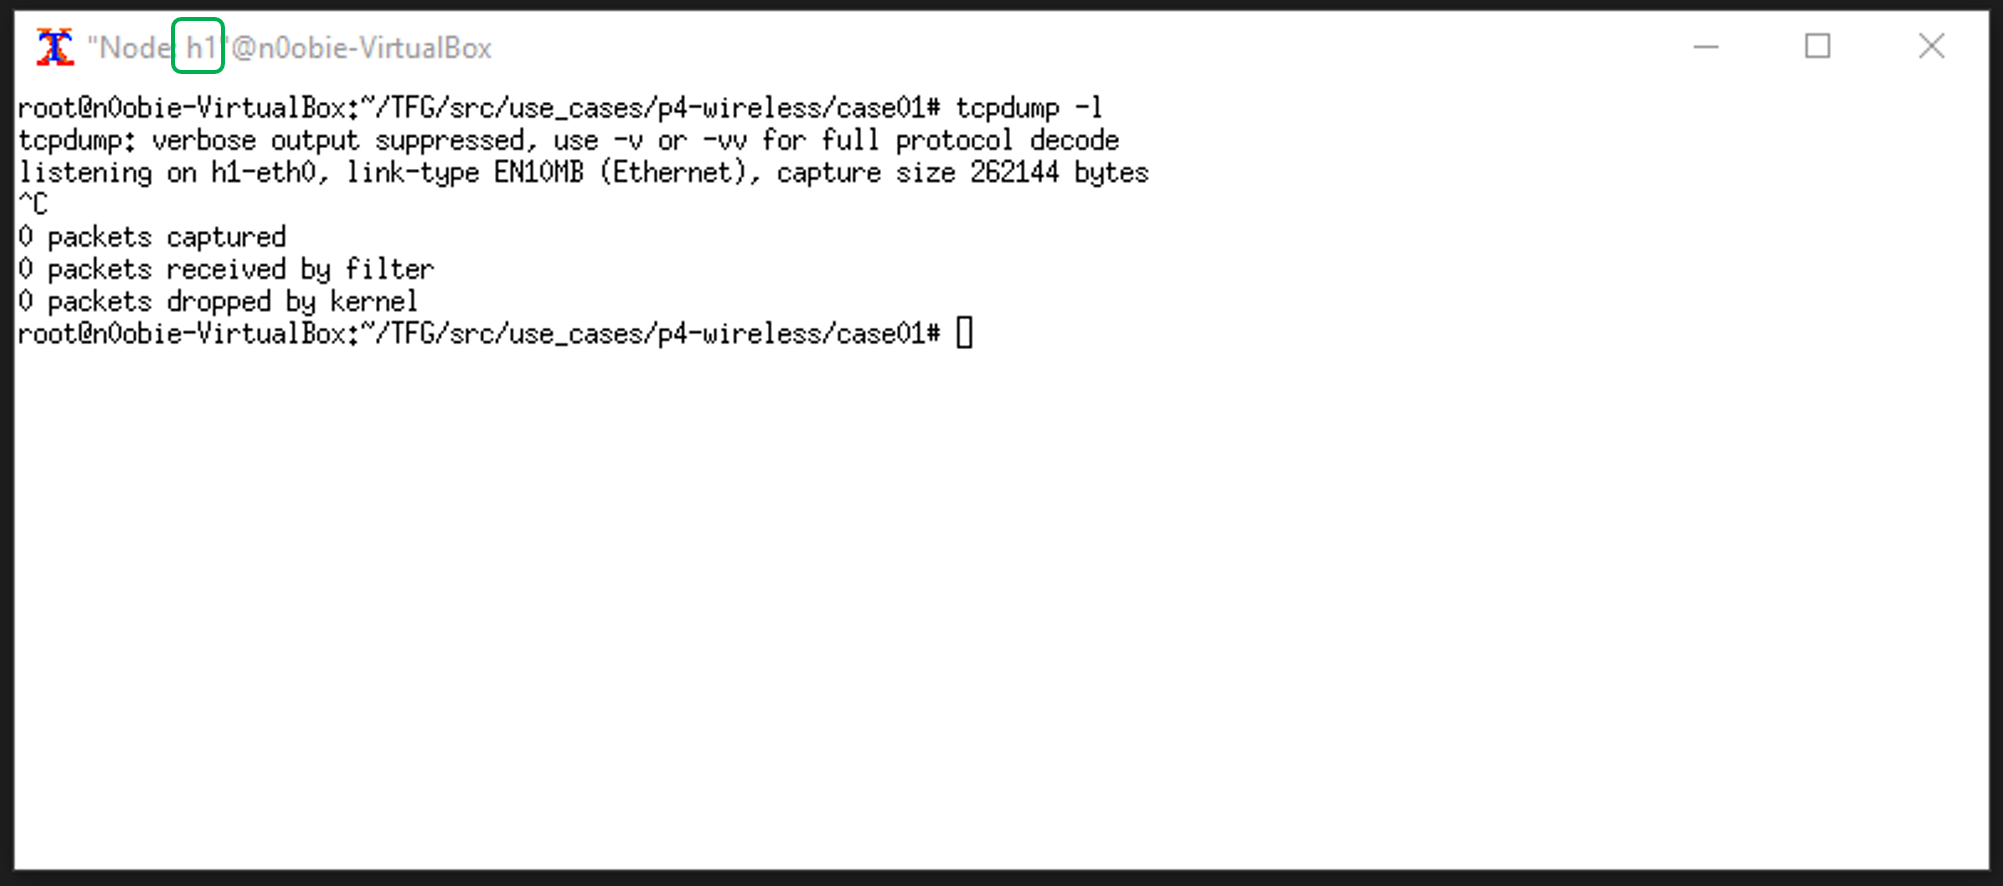
\includegraphics[width=14cm]{archivos/img/dev/p4-wifi/case01/demo_case01_2_edited.png}
    \caption{Comprobación de funcionamiento (Sniffer) del Case01 - P4 Wireless}
    \label{fig:case01_p4_wifi_func2}
\end{figure}